\documentclass[aspectratio=169,10pt,t,german,xcolor=table]{beamer}
\usepackage{../../common/beamer-cgs-lecture}

\title{Gem Illuminator}
\author{Pascal Lange, Sebastian Koall, Jennifer Stamm}
\institute{\translate{Hasso Plattner Institute}}
\date{WiSe~2014/2015}

\subtitle{Game Programming}
\titlegraphic{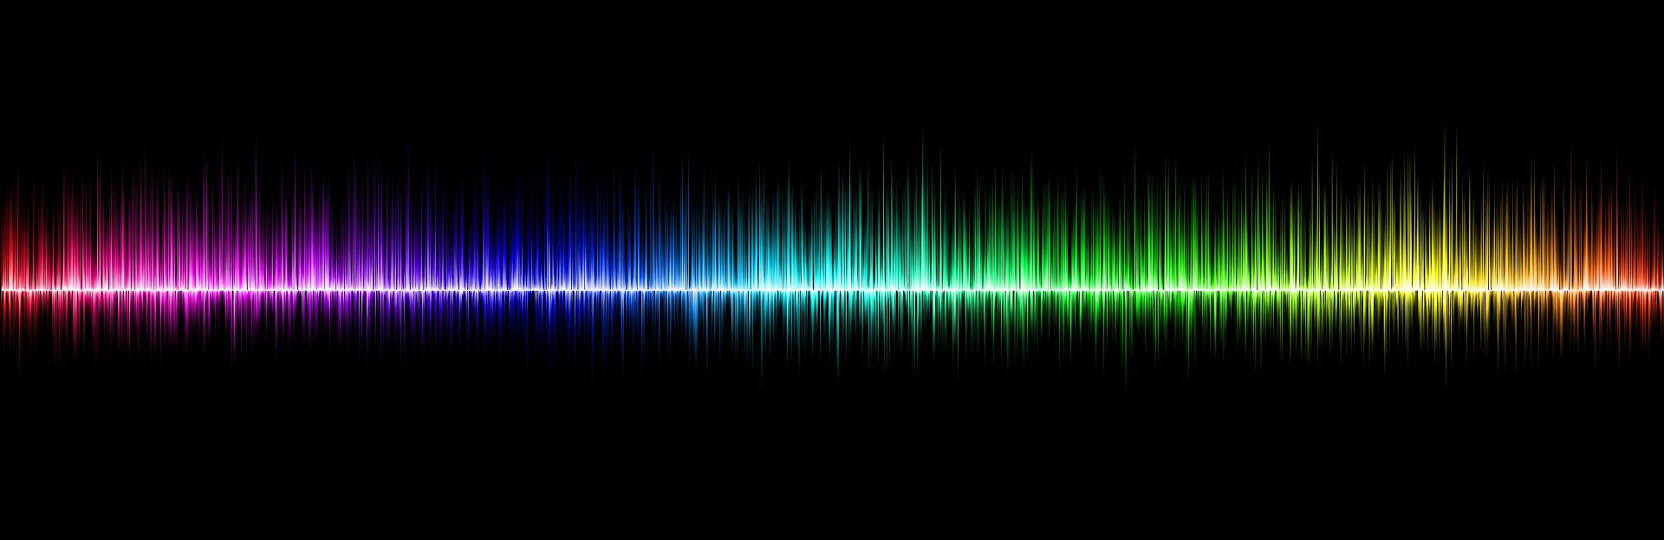
\includegraphics[width=\linewidth]{images/teaser}}

\begin{document}

\slidetitle
\section*{Zwischenstandspräsentation}

\begin{frame}{Demo}
	%TODO Aktueller Screenshot/Video
	\begin{figure}
		\centering
		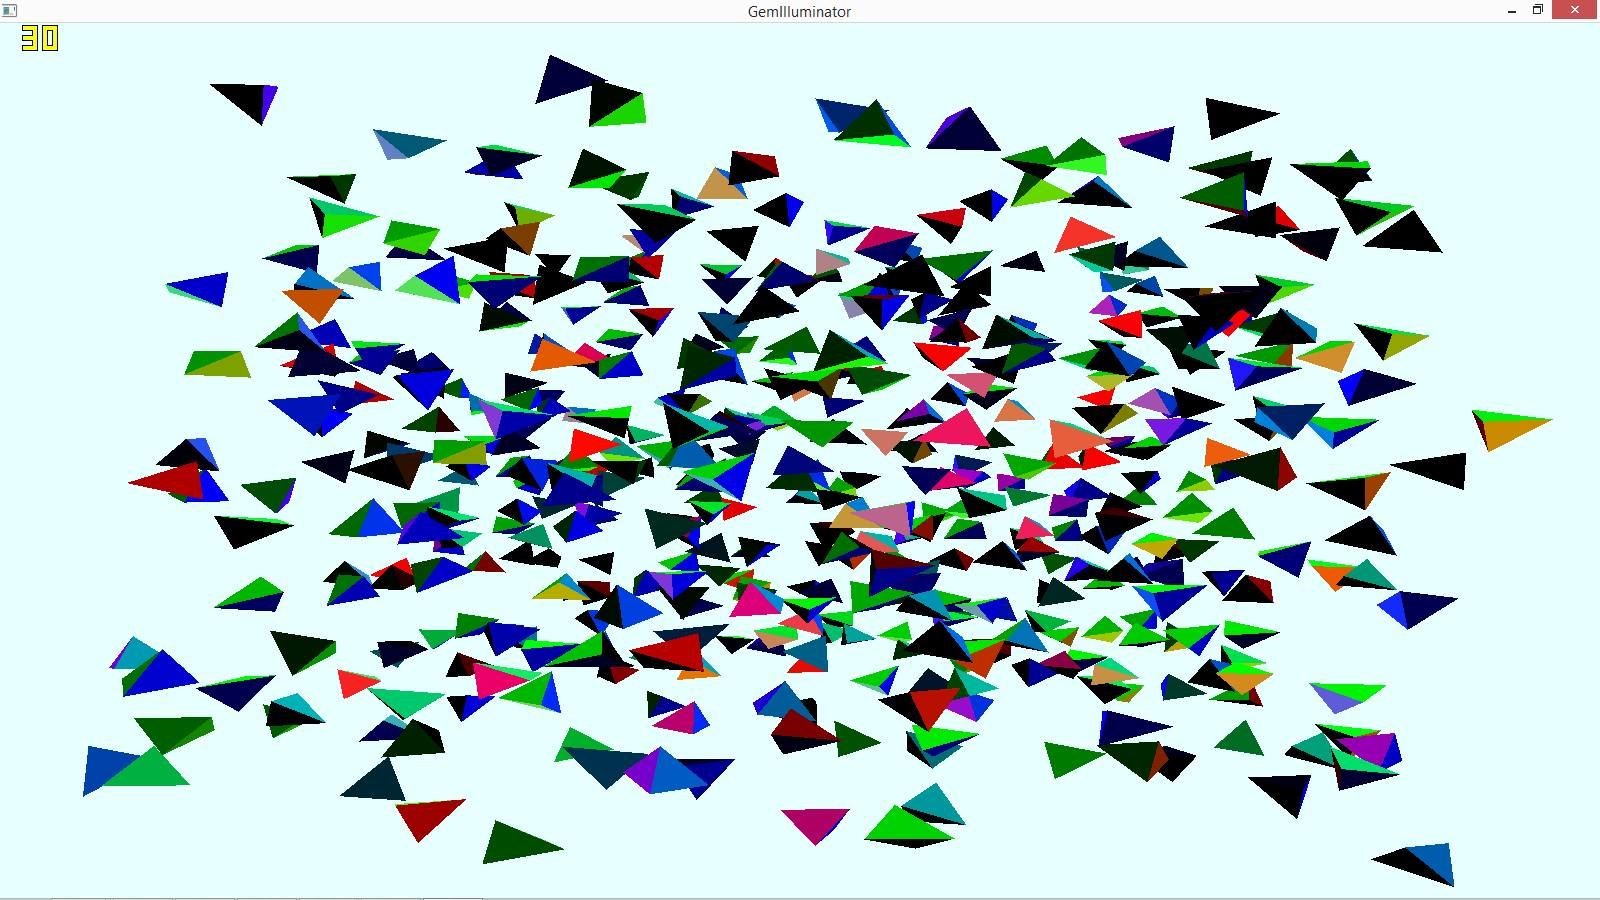
\includegraphics[width=\textwidth, height=0.7\textheight, keepaspectratio]{images/500_gems_intel}
	\end{figure}
\end{frame}


\begin{frame}{Architektur -- C++}
	\begin{figure}
		\centering
		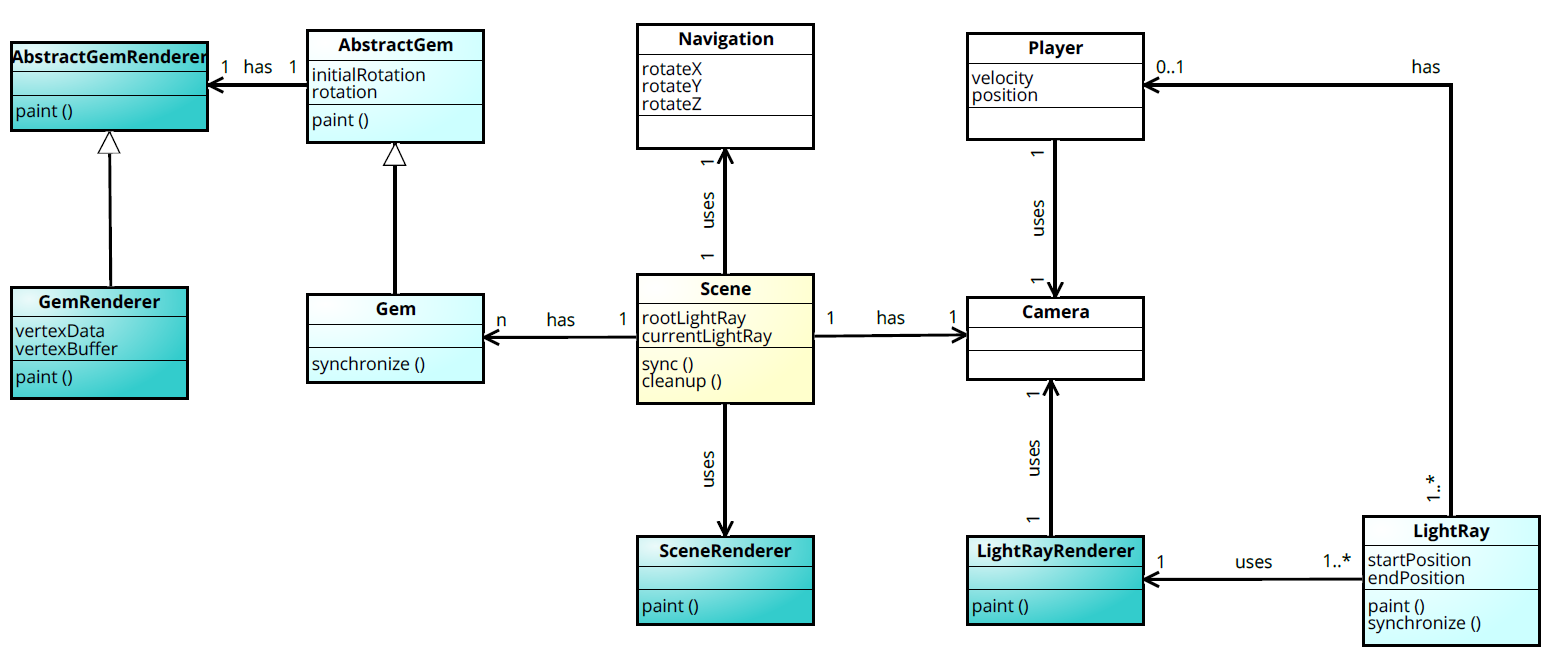
\includegraphics[width=\textwidth, height=\textheight, keepaspectratio]{images/klassendiagramm}
	\end{figure}
\end{frame}


\slideonetoone
{Herausforderungen}
{	
	\begin{figure}
		\centering
		\begin{subfigure}{\textwidth}
			\centering
			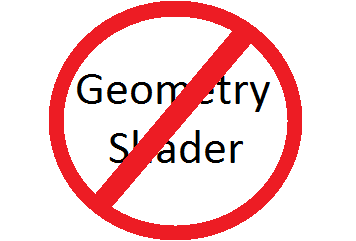
\includegraphics[width=\textwidth, height=0.3\textheight, keepaspectratio]{images/nogeometry}
			\caption{Normalenberechnung}
		\end{subfigure}
		\begin{subfigure}{\textwidth}
			\centering
			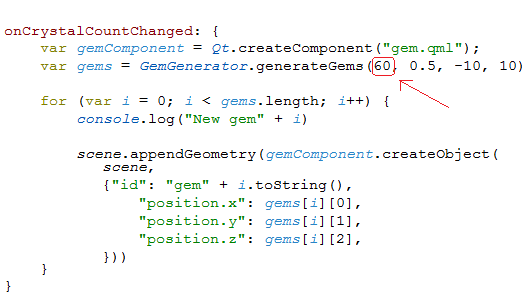
\includegraphics[width=\textwidth, height=0.3\textheight, keepaspectratio]{images/60max}
			\caption{QML-Propertylists.append???}
		\end{subfigure}
	\end{figure}
}
{
	\begin{figure}
		\centering
		\begin{subfigure}{\textwidth}
			\centering
			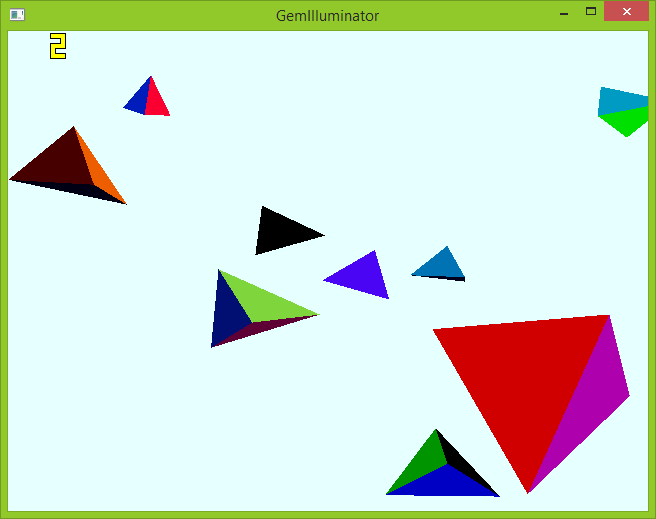
\includegraphics[width=\textwidth, height=0.3\textheight, keepaspectratio]{images/lowFPS}
			\caption{Niedrige Framerate}
		\end{subfigure}
		\begin{subfigure}{\textwidth}
			\centering
			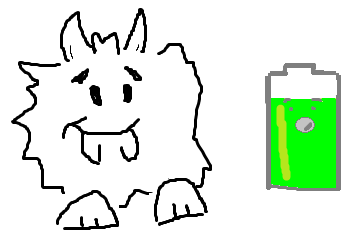
\includegraphics[width=\textwidth, height=0.3\textheight, keepaspectratio]{images/akkufresser}
			\caption{Akkufresser}
		\end{subfigure}
	\end{figure}
}



\slideonetoone
{Lösungskonzepte}
{	
	\begin{figure}
		\centering
		\begin{subfigure}{\textwidth}
			\centering
			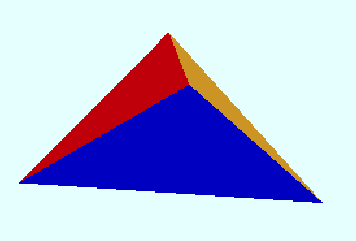
\includegraphics[width=\textwidth, height=0.3\textheight, keepaspectratio]{images/nogeometry2}
			\caption{Normalenberechnung}
		\end{subfigure}
		\begin{subfigure}{\textwidth}
			\centering
			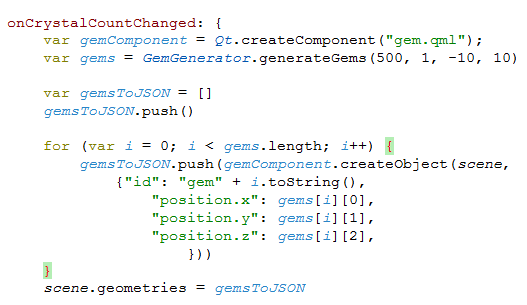
\includegraphics[width=\textwidth, height=0.3\textheight, keepaspectratio]{images/60max2}
			\caption{QML-Propertylists.append???}
		\end{subfigure}
	\end{figure}
}
{
	\begin{figure}
		\centering
		\begin{subfigure}{\textwidth}
			\centering
			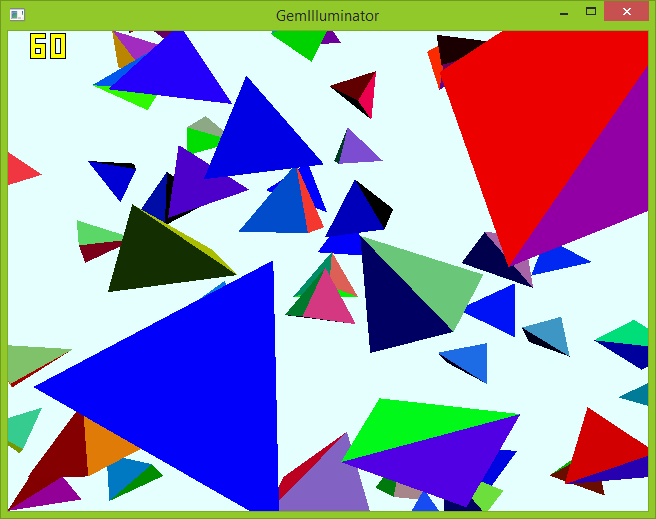
\includegraphics[width=\textwidth, height=0.3\textheight, keepaspectratio]{images/highFPS}
			\caption{Niedrige Framerate}
		\end{subfigure}
		\begin{subfigure}{\textwidth}
			\centering
			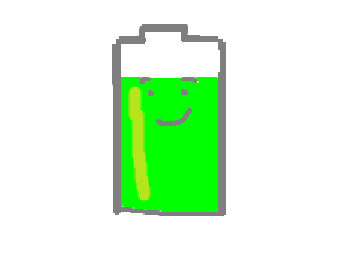
\includegraphics[width=\textwidth, height=0.3\textheight, keepaspectratio]{images/akkufresser2}
			\caption{Akkufresser}
		\end{subfigure}
	\end{figure}
}

\lstdefinelanguage{JavaScript}{
  keywords={typeof, new, true, false, catch, function, return, null, catch, switch, var, if, in, while, do, else, case, break},
  keywordstyle=\color{blue}\bfseries,
  ndkeywords={class, export, boolean, throw, implements, import, this},
  ndkeywordstyle=\color{darkgray}\bfseries,
  identifierstyle=\color{black},
  sensitive=false,
  comment=[l]{//},
  morecomment=[s]{/*}{*/},
  commentstyle=\color{purple}\ttfamily,
  stringstyle=\color{red}\ttfamily,
  morestring=[b]',
  morestring=[b]"
}

\begin{frame}
{Detaillierter Lösungsansatz -- Akkufresser}
	\lstinputlisting[language=JavaScript, breaklines, firstline=1, lastline=24]{code/active.js}
\end{frame}
\begin{frame}
{Detaillierter Lösungsansatz -- Akkufresser}
	\lstinputlisting[language=JavaScript, breaklines, firstline=25, lastline=46, firstnumber=25]{code/active.js}
\end{frame}




\begin{frame}{Milestones}
	\begin{itemize}
		\definecolor{evap@lightgreen}{HTML}{bbd154}
		
		\definecolor{evap@darkgreen}{HTML}{88be4a}
		
		\definecolor{evap@yellow}{HTML}{eee258}

		\item \textcolor{evap@lightgreen}{Ende November\\
			Prototyp mit Landschafts-Generierung abstrakter \glqq Kristall\grqq -Objekte im Raum. Idealerweise können wir bereits das zu steuernde Objekt ausfindig machen.}
			
		\item \textcolor{evap@yellow}{Zwischenstandspräsentation\\
			Vollständige Implementierung der Steuerung und Berechnung des übernächsten Objekts, auf das die Strahlen treffen würden.}
			
		\item Ende der Weihnachtsferien\\
			Umstellung von Listen auf Baumstrukturen. Kollisionserkennung.
		\item Early Access Convention\\
			Auswahl des Kristalls, auf den das Lichtbündel trifft. (Erster Lichteffekt: Spekulare Reflektion.)
	\end{itemize}
\end{frame}

\begin{frame}{Offene Fragen}
	\begin{itemize}
		\item Was passiert, wenn ein Lichtstrahl auf keinen Kristall trifft?
		\item[]
		\item Woran erkennt man den Kristall, den man steuern kann?
		\item[]
		\item Wie soll der Hintergrund aussehen?
		\item[]
		\item Was verhalten sich mehrere Lichtstrahlen?
		\item[]		
		\item Sound, wer, wie, wo, was?
		\item[]		
		\item Und wer ist eigentlich diese Usability?
	\end{itemize}

\end{frame}

%\begin{frame}[allowframebreaks]{Bibliographie}
  \bibliographystyle{apalike}
  \bibliography{../../references}
  \vfill
\end{frame}

\end{document}
